%\title{LaTeX Portrait Poster Template}
%%%%%%%%%%%%%%%%%%%%%%%%%%%%%%%%%%%%%%%%%
% a0poster Portrait Poster
% LaTeX Template
% Version 1.0 (22/06/13)
%
% The a0poster class was created by:
% Gerlinde Kettl and Matthias Weiser (tex@kettl.de)
% 
% Adapter by Jens Buysse for Hogeschool Gent
% This template has been downloaded from:
% http://www.LaTeXTemplates.com
%
% License:
% CC BY-NC-SA 3.0 (http://creativecommons.org/licenses/by-nc-sa/3.0/)
%
%%%%%%%%%%%%%%%%%%%%%%%%%%%%%%%%%%%%%%%%%

%----------------------------------------------------------------------------------------
%	PACKAGES AND OTHER DOCUMENT CONFIGURATIONS
%----------------------------------------------------------------------------------------

\documentclass[a0,portrait]{a0poster}

\usepackage{multicol} % This is so we can have multiple columns of text side-by-side
\columnsep=100pt % This is the amount of white space between the columns in the poster
\columnseprule=3pt % This is the thickness of the black line between the columns in the poster

\usepackage[svgnames]{xcolor} % Specify colors by their 'svgnames', for a full list of all colors available see here: http://www.latextemplates.com/svgnames-colors

\usepackage{times} % Use the times font
%\usepackage{palatino} % Uncomment to use the Palatino font

\usepackage{graphicx} % Required for including images
\graphicspath{{figures/}} % Location of the graphics files
\usepackage{booktabs} % Top and bottom rules for table
\usepackage[font=small,labelfont=bf]{caption} % Required for specifying captions to tables and figures
\usepackage{amsfonts, amsmath, amsthm, amssymb} % For math fonts, symbols and environments
\usepackage{wrapfig} % Allows wrapping text around tables and figures
\usepackage[export]{adjustbox}

\begin{document}

%----------------------------------------------------------------------------------------
%	POSTER HEADER 
%----------------------------------------------------------------------------------------

% The header is divided into two boxes:
% The first is 75% wide and houses the title, subtitle, names, university/organization and contact information
% The second is 25% wide and houses a logo for your university/organization or a photo of you
% The widths of these boxes can be easily edited to accommodate your content as you see fit

\begin{minipage}[t]{0.75\linewidth}
\VeryHuge \color{HoGentAccent1} \textbf{Analyse, architectuur en proof-of-concept van een beveiligde omgeving voor het afnemen van computerexamens op eigen laptop} \color{Black}\\ % Title
\\
\huge \textbf{Balliu Benoit, Van Vreckem Bert}\\[0.5cm] % Author(s)
\huge Hogeschool Gent, Valentin Vaerwyckweg 1, 9000 Gent\\[0.4cm] % University/organization
\Large \texttt{benoit.balliu.y9010@student.hogent.be} \\
\end{minipage}
%
\begin{minipage}[t]{0.25\linewidth}

\includegraphics[width=13cm,right]{figures/HOGENT_Logo_Pos_rgb.png} 

\end{minipage}

\vspace{1cm} % A bit of extra whitespace between the header and poster content

%----------------------------------------------------------------------------------------

\begin{multicols}{2} % This is how many columns your poster will be broken into, a portrait poster is generally split into 2 columns

%----------------------------------------------------------------------------------------
%	ABSTRACT
%----------------------------------------------------------------------------------------

\color{HoGentAccent1} % Navy color for the abstract

\begin{abstract}
\bigskip
Deze bachelorproef is gemaakt in opdracht van Hogeschool Gent, zij willen graag hun huidig systeem om examens op computer af te nemen moderniseren. Momenteel beheert de afdeling Systeembeheer van Hogeschool Gent een groot aantal desktops en softwarepakketten in combinatie met NetSupport School, maar daar loopt af en toe iets mis. Het komt wel vaker voor dat examens niet automatisch opgehaald kunnen worden of examens niet door kunnen gaan omdat de juiste software niet ge\"{i}nstalleerd is. 

Voor het nieuwe systeem wil Hogeschool Gent de mogelijkheid van bring-your-own-device examens onderzoeken. Dit is een systeem waarbij de studenten de examens afleggen op hun eigen laptop. De grootste uitdaging van dergelijk systeem is deze laptops genoeg beveiligen tegen fraude. Voor dit onderzoek werd uitdrukkelijk gevraagd om te onderzoeken of zo een systeem haalbaar is zonder dat studenten hiervoor speciale software op hun systeem dienen te installeren.

Na het onderzoeken van enkele systemen is er besloten een proof-of-concept op te stellen van een beveiligde netwerkomgeving. Hoewel deze omgeving alle vormen van fraude via het internet voorkomt, kan er niet uitgesloten worden dat een student opgeloste oefeningen of een cursus op zijn laptop heeft staan. Dit systeem voldoet dus niet aan de eisen van de Hogeschool Gent want het zou een stuk minder veilig zijn dan de methode die ze vandaag hanteert. 

De belangrijkste conclusie van dit onderzoek is dat fraude op laptops van de studenten niet kan uitgesloten worden zonder dat er speciale software (bijvoorbeeld monitoring-software) ge\"{i}nstalleerd wordt. Het lijkt mij daarom interessant om het onderzoek naar bring-your-own-device examens opnieuw te voeren met andere uitgangspunten. Mogelijks lijdt een aangepast onderzoek tot nieuwe inzichten.
\end{abstract}
%----------------------------------------------------------------------------------------
%	INTRODUCTION
%----------------------------------------------------------------------------------------

\color{HoGentAccent1} 
 \section*{Introductie}
 \color{black}
 \color{black}
 
 Momenteel worden de meeste computerexamens op Hogeschool Gent in een beveiligde omgeving op een computer van de hogeschool afgenomen. Deze methodiek heeft enkele nadelen. De voornaamste is de onbetrouwbaarheid van de omgeving. Wanneer een systeem zo'n kritieke functie heeft, is er slechts een kleine foutenmarge, het huidige systeem overschrijdt deze marge.  Verder zorgt het systeem ook voor een hoge kost, de hogeschool moet een groot aantal computers ter beschikking stellen en deze moeten beschikken over software eigen aan het examen, en monitoringsoftware zodat de examens in een beveiligde omgeving afgelegd kunnen worden. \\ In deze bachelorproef onderzoeken we de haalbaarheid van een beveiligde omgeving waar studenten computerexamens op hun eigen laptop kunnen afleggen. Deze beveilige omgeving moet fraude uitsluiten. \\
 
 



%----------------------------------------------------------------------------------------
%	GEOLOGY
%----------------------------------------------------------------------------------------

\color{Black} % DarkSlateGray color for the rest of the content
\color{HoGentAccent1} 
\section*{Mogelijke opstellingen}
\color{black}

Het invoeren van BYOD examens kan op verschillende manieren. Daarom is er een scope vastgesteld voor dit onderzoek. De implementatie van BYOD examens moet hetzelfde zijn voor de 3 meest gangbare besturingssystemen (Linux, MacOs en Windows) en het is niet de bedoeling, dat een student specifieke software moet installeren (voor monitoring of internet filtering e.d.). Deze scope limiteert het aantal mogelijke implementaties. In dit onderzoek zijn er 4 manieren om BYOD examens te faciliteren onderzocht, namelijk: \\

\begin{itemize} 
	\item \textbf{Desktop virtualisatie via een cloudprovider}
	\item \textbf{Beveiligde, configureerbare netwerkomgeving om internettoegang tot niet-toegestane sites vanop laptops tegen te gaan.	}
	\item \textbf{Safe Exam Browser }
	\item \textbf{Televic AssessmentQ / AVIDAnet Lite}
\end{itemize}
\bigskip
 Na wat eigen onderzoek hierrond, bleek dat de laatste 2 in deze lijst  out of scope vielen. Deze zijn enkel bruikbaar voor examens die louter uit vragenlijsten bestaan. Voor beide systemen is er een extra programma nodig dat op de laptop van de student ge\"{i}nstalleerd zou moeten worden. Bij een safe exam browser moet er buiten de browser zelf ook nog een kiosk-applicatie ge\"{i}nstalleerd worden, die bepaalde systeemfuncties kan blokkeren tijdens een examen  Kiosk software is een allesomvattende term voor software waarbij het systeem afgeschermd is van interactie door gebruikers binnen een bepaalde scope. Televic assessmentQ maakt op zijn beurt gebruik van zo een Safe Exam Browser. \\

\textbf{Desktopvirtualisatie via een cloudprovider}

Een lector bouwt een examen-image vanaf een template. Hij installeert op dergelijke template de nodige software voor het examen, plaatst de nodige files op het systeem (GitHub Classroom) en test of alles werkt.  Daarna wordt er via een tool (Packer e.d.) een image van die machine gemaakt.  Bij aanvang van het examen vraagt elke student een kopie van die virtuele machine aan via een cloudprovider (Amazon AWS, Microsoft Azure e.d.) met credentials die door de school worden aangeleverd. De lector kan via de firewallinstellingen ook beslissen of de studenten op het internet mogen en indien toegestaan welke sites ze mogen bezoeken. Na het verwerven van de toegang tot hun persoonlijke machine krijgen ze, zoals bij een normaal examen, tijd om de vragen te beantwoorden. Wanneer ze daarmee klaar zijn kunnen ze hun examen via GitHub Classroom indienen en wordt de machine terug verwijderd. \\



\textbf{Beveiligde, configureerbare netwerkomgeving om internettoegang tot niet-toegestane sites vanop laptops tegen te gaan.	} 

Hierover is meer te lezen in de volgende sectie.

\bigskip

\bigskip


\color{HoGentAccent1} 
\section*{Finale opstelling}
\color{black}

\begin{center}\vspace{1cm}
	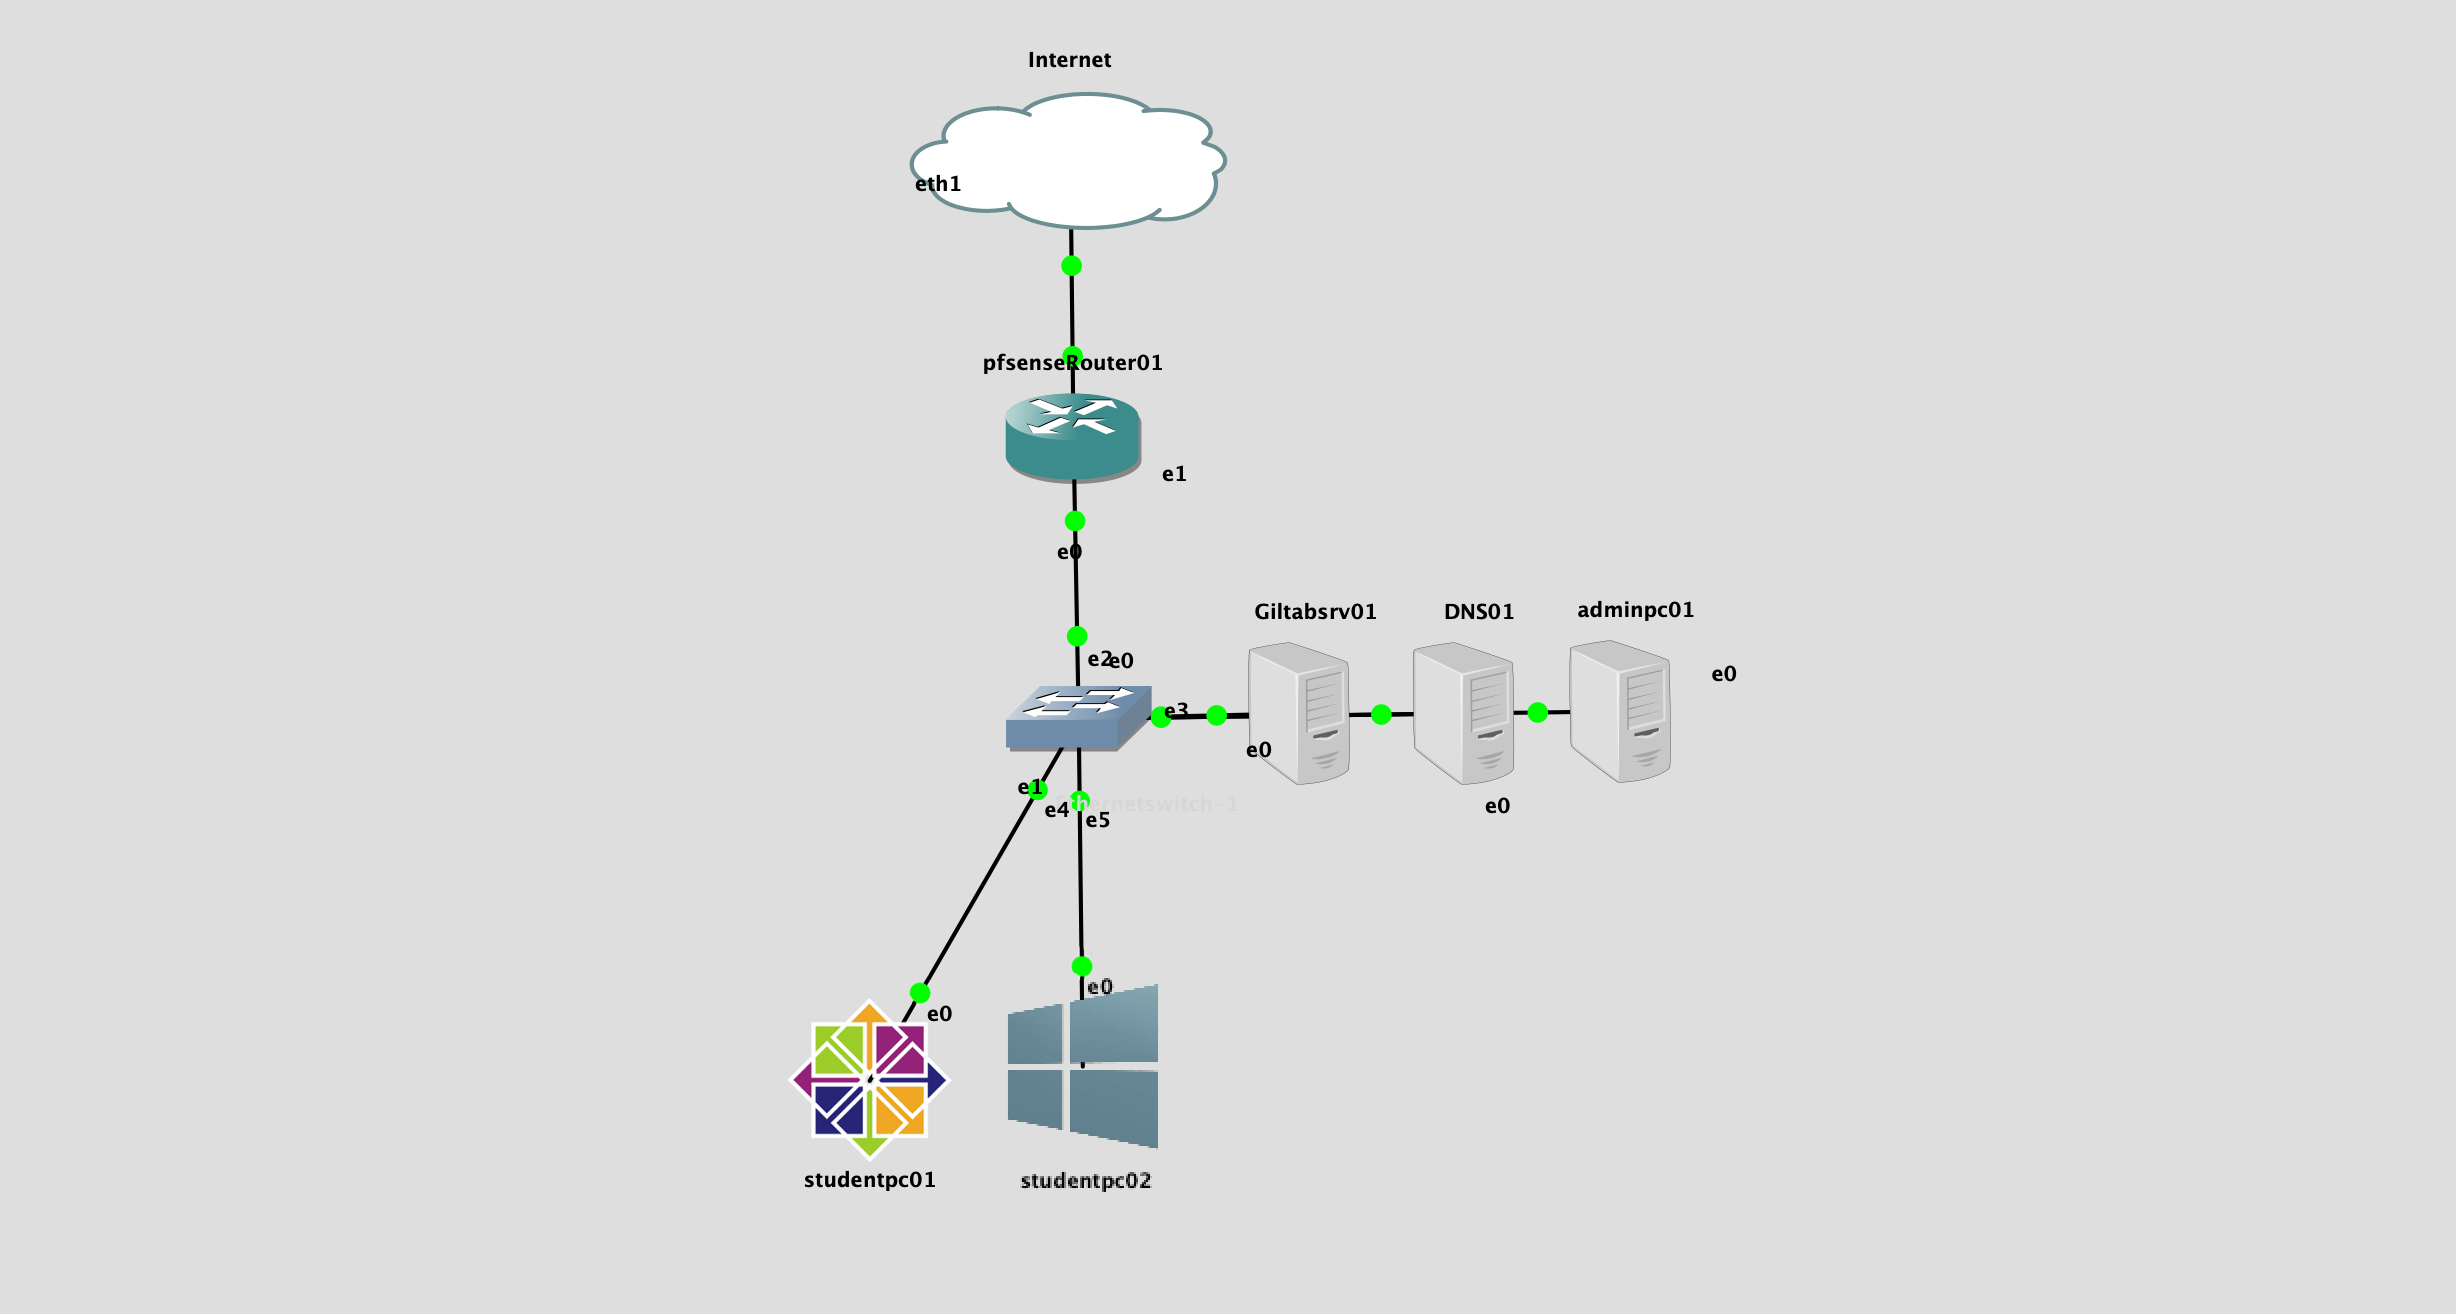
\includegraphics[width=1.0\linewidth]{gns3FinalPoC}
	\label{1}
	\captionof{figure}{\color{HoGentAccent5} Eindelijke opstelling, hier voorgesteld in GNS3}
\end{center}\vspace{1cm}

De opstelling van de  proof-of-concept, die u terug kan vinden op figuur 1, bestaat uit:
\begin{itemize}
	\item pfSense router en firewall
	\item CentOS server met een dnsmasq DNS en DHCP Server
	\item CentOS server met Gitlab Community Edition ge\"{\i}nstalleerd.
	\item Switch
	\item End devices (laptops)
\end{itemize}
\bigskip

\textbf{Functionaliteiten}

Hier volgt een opsomming van alle functionaliteiten die een dergelijke opstelling bevat.

\begin{itemize}
	\item Alle admin systemen zijn beveiligd volgens een Baseline gebaseerd op de CIS Guidelines (Zie bijlage).
	\item Het opzetten van de omgeving voor een examen wordt grotendeels door Ansible gedaan.
	\item Een lector kan dankzij het gebruiksvriendelijke Ansible zijn examenomgeving vlot zelf configureren.
	\item De studenten kunnen enkel browsen naar websites die toegestaan zijn door de lectoren.
	\item Beveiliging op zowel de firewall en DNS zorgen ervoor dat studenten geen VPN-verbinding kunnen maken of een andere DNS Server kunnen gebruiken.
	\item Studenten kunnen hun examen van de lokale Gitlab server halen en na het examen indienen via Gitlab
	\item Er wordt gemonitord of studenten niet met andere netwerken verbinden.
\end{itemize}
\bigskip

\textbf{Ontbrekende functionaliteiten}

Deze proof-of-concept is geen ideale oplossing voor het nieuwe examensysteem, maar wel de best mogelijke oplossing binnen dit onderzoek.
Toch blijft er een functionaliteit over die voor sommige examens een nice-to-have is en voor andere een must-have, namelijk: 

Studenten hebben volledige toegang tot documenten op hun eigen laptop. Indien zij reeds gemaakte oefeningen, opgeloste voorbeeldexamens of vorige versies van examens bij zouden hebben, is het mogelijk dat zij een oneerlijk voordeel krijgen tegenover andere studenten. Volgens een lector die programmeerexamens afneemt, maakt dat voor examens zoals "Object-Geori\"{e}nteerd Programmeren III" minder uit in vergelijking met "Object-Geori\"{e}nteerd Programmeren I", waarbij het voor die lector noodzakelijk is dat studenten geen toegang hebben tot alle oefeningen.




%------------------------------------------------



\color{HoGentAccent1} 
\section*{Conclusie}
\color{black}

Uit het onderzoek naar een nieuwe, BYOD, examenomgeving is gebleken dat dergelijke omgeving nooit genoeg beveiligd kan worden tegen fraude. Dit natuurlijk binnen de scope die aan het onderzoek gegeven is, namelijk, het is niet de bedoeling dat er software op apparaten van de studenten ge\"{\i}nstalleerd wordt. De beveiligde netwerkomgeving, zoals voorgesteld in in de vorige sectie, is de enige omgeving die tegen fraude via het internet beschermt. In dergelijke omgeving is er geen controle op de documenten waarover de student beschikt. De nieuwe examenomgeving zou minstens het zelfde niveau van beveiliging als het huidige NetSupport School systeem moeten halen.  



%----------------------------------------------------------------------------------------
%	FORTHCOMING RESEARCH
%----------------------------------------------------------------------------------------
\color{HoGentAccent1} 
\section*{Toekomstig onderzoek}
\color{black}

Het principe van bring-your-own-device examens is wel interessant gebleken, vooral door de lagere kosten en de kleinere administratieve overhead. Het zou daarom opportuun zijn om dit onderzoek te hernemen, met een gewijzigde scope. Indien bij het onderzoeken van een BYOD examenomgeving, het installeren van (kiosk)software op apparaten van studenten toegestaan is, kan dergelijk onderzoek mogelijks een ander resultaat opleveren.

%----------------------------------------------------------------------------------------

\end{multicols}
\end{document}